% Options for packages loaded elsewhere
\PassOptionsToPackage{unicode}{hyperref}
\PassOptionsToPackage{hyphens}{url}
\PassOptionsToPackage{dvipsnames,svgnames*,x11names*}{xcolor}
%
\documentclass[
  spanish,
]{article}
\usepackage[sfdefault,lining]{FiraSans}
\usepackage{amsmath}
\usepackage{ifxetex,ifluatex}
\ifnum 0\ifxetex 1\fi\ifluatex 1\fi=0 % if pdftex
  \usepackage[T1]{fontenc}
  \usepackage[utf8]{inputenc}
  \usepackage{textcomp} % provide euro and other symbols
  \usepackage{amssymb}
\else % if luatex or xetex
  \usepackage{unicode-math}
  \defaultfontfeatures{Scale=MatchLowercase}
  \defaultfontfeatures[\rmfamily]{Ligatures=TeX,Scale=1}
\fi
% Use upquote if available, for straight quotes in verbatim environments
\IfFileExists{upquote.sty}{\usepackage{upquote}}{}
\IfFileExists{microtype.sty}{% use microtype if available
  \usepackage[]{microtype}
  \UseMicrotypeSet[protrusion]{basicmath} % disable protrusion for tt fonts
}{}
\makeatletter
\@ifundefined{KOMAClassName}{% if non-KOMA class
  \IfFileExists{parskip.sty}{%
    \usepackage{parskip}
  }{% else
    \setlength{\parindent}{0pt}
    \setlength{\parskip}{6pt plus 2pt minus 1pt}}
}{% if KOMA class
  \KOMAoptions{parskip=half}}
\makeatother
\usepackage{xcolor}
\IfFileExists{xurl.sty}{\usepackage{xurl}}{} % add URL line breaks if available
\IfFileExists{bookmark.sty}{\usepackage{bookmark}}{\usepackage{hyperref}}
\hypersetup{
  pdftitle={Las transformaciones químicas de la materia},
  pdfauthor={Guillermo Martínez Gutiérrez},
  pdflang={es-ES},
  colorlinks=true,
  linkcolor=Maroon,
  filecolor=Maroon,
  citecolor=Blue,
  urlcolor=Blue,
  pdfcreator={LaTeX via pandoc}}
\urlstyle{same} % disable monospaced font for URLs
\usepackage[a4paper,headheight=10mm,headsep=10mm,top=30mm]{geometry}
\usepackage{graphicx}
\makeatletter
\def\maxwidth{\ifdim\Gin@nat@width>\linewidth\linewidth\else\Gin@nat@width\fi}
\def\maxheight{\ifdim\Gin@nat@height>\textheight\textheight\else\Gin@nat@height\fi}
\makeatother
% Scale images if necessary, so that they will not overflow the page
% margins by default, and it is still possible to overwrite the defaults
% using explicit options in \includegraphics[width, height, ...]{}
\setkeys{Gin}{width=\maxwidth,height=\maxheight,keepaspectratio}
% Set default figure placement to htbp
\makeatletter
\def\fps@figure{htbp}
\makeatother
\setlength{\emergencystretch}{3em} % prevent overfull lines
\providecommand{\tightlist}{%
  \setlength{\itemsep}{0pt}\setlength{\parskip}{0pt}}
\setcounter{secnumdepth}{-\maxdimen} % remove section numbering
\everymath{\displaystyle}
\ifxetex
  % Load polyglossia as late as possible: uses bidi with RTL langages (e.g. Hebrew, Arabic)
  \usepackage{polyglossia}
  \setmainlanguage[]{}
\else
  \usepackage[shorthands=off,main=spanish]{babel}
\fi
\ifluatex
  \usepackage{selnolig}  % disable illegal ligatures
\fi

\title{Las transformaciones químicas de la materia}
\author{Guillermo Martínez Gutiérrez}
\date{Mayo 2024}


% % MODIFICATIONS MADE BY ME

% MODIFICATIONS MADE BY ME

%\usepackage[sfdefault,lining]{FiraSans} %% option 'sfdefault' activates Fira Sans as the default text font
\usepackage[fakebold]{firamath-otf}
\renewcommand*\oldstylenums[1]{{\firaoldstyle #1}}
\setmathfont{Fira Math}


\usepackage{siunitx}
\sisetup{detect-all}
\sisetup{
    exponent-product        = \cdot,
    per-mode                = reciprocal,
    output-decimal-marker   = {,},
    group-digits            = integer,
    %text-celsius            = ^^b0\kern -\scriptspace C, % soluciona problemas con el símbolo de grados
    %math-celsius            = ^^b0\kern -\scriptspace C,
    list-final-separator    = { y },
    list-pair-separator     = { y },
    range-phrase            = { \translate{to (numerical range)} },
    qualifier-mode          = brackets,
    separate-uncertainty    = true,
    multi-part-units        = single,
    retain-explicit-plus    = true,
}
\DeclareSIUnit\torr{torr}
\DeclareSIUnit\atm{atm}
\DeclareSIUnit\molar{M}
\DeclareSIUnit\M{\molar}
\DeclareSIUnit\kcal{kcal}
\DeclareSIUnit\cal{cal}
\DeclareSIUnit\mol{\mole}
\DeclareSIUnit\uma{u}
\DeclareSIUnit\h{\hour}
\DeclareSIUnit\hora{\hour}
\DeclareSIUnit\min{\minute}
\DeclareSIUnit\minuto{\minute}


% Alternativa de configuración para expresar unidades como fracciones
% en la forma mol/L (en lugar de con exponentes negativos)
\sisetup{
    per-mode                  = symbol,
    per-symbol                = /,
    bracket-unit-denominator  = true,
}
\usepackage{chemfig, chemformula}
  \setchemfig{atom sep=2em}
  \setchemformula{frac-style = nicefrac}
\usepackage[no-files]{xsim}
  \loadxsimstyle{ged}
  \xsimsetup{
    % path                  = {xsim},
    exercise/template     = {gedmargin},
    exercise/name         = {},
    exercise/print        = {true},
    solution/template     = {gedsolution},
    solution/name         = {Solución: },
    solution/print        = {false},
    % exercise/within       = section,
    % exercise/the-counter  = \thesection.\arabic{exercise},
  }
\usepackage{icomma}
\usepackage[gen]{eurosym}
\usepackage{multicol}
\usepackage{fancyhdr}
\usepackage{tabularray}
\pagestyle{fancy}

\addtolength{\headwidth}{\marginparsep}
\addtolength{\headwidth}{\marginparwidth}
\renewcommand{\headwidth}{1.1\linewidth}
\fancyheadoffset[LR]{0.1\linewidth}
\fancyhead{

  \begin{tblr}{
%    width=1.2\linewidth,
    colspec = {Q[c,h]l|X[c]|c|},
    stretch = 0,
    rowsep = 0pt,
    column{1} = {colsep=0pt},
    column{2} = {leftsep=0pt, font=\itshape},
    rows = {font=\footnotesize},
    hlines = {3-4}{0.5pt},
%    vline{2-5} = {1pt},
  }
    
\includegraphics{D:/DOCENCIA/banco-de-ejercicios/.pandoc-config/assets/logo_IES_astures.png} & {Dpto. de \\ \emph{Física y Química}} & { {\normalsize } \\ } & { \\ Curso 2023-24} \\
  \end{tblr}
}
\renewcommand{\headrulewidth}{0pt}



% Tikz & pgfplots
\usepackage{pgfplots}
\pgfplotsset{compat=1.9}
\usetikzlibrary{shapes.geometric}
\pgfplotsset{posicion tiempo/.style={
  xlabel={Tiempo [s]},
  ylabel={Posición [m]},
  width=4cm,
  axis lines=left,
  axis x line=middle,
  xtick distance=2,
  ytick distance=20,
  %minor tick num=4,
  grid=both,
  grid style={solid,lightgray},
  minor grid style={solid,very thin},
  font=\scriptsize,
  label style={font=\tiny}
}}


% END MODIFICATIONS


% Definitions
\newcommand{\entalpia}[1][]{\Delta _{#1} H\textdegree}
\newcommand{\entalpiade}[2][]{\Delta _{#1} H\textdegree \left[\ch{#2}\right]}
\newcommand{\entropia}[1][]{\Delta _{#1} S\textdegree}
\newcommand{\entropiade}[2][]{\Delta _{#1} S\textdegree \left[\ch{#2}\right]}
\newcommand{\Gibbs}[1][]{\Delta _{#1} G\textdegree}
\newcommand{\Gibbsde}[2][]{\Delta _{#1} G\textdegree \left[\ch{#2}\right]}
\newcommand{\conc}[2][]{[ \ch{#2} ]_{#1}}
\newcommand{\pparcial}[1]{p_{\ch{#1}}}
\newcommand{\potE}[2]{E\textdegree (\ch{#1}/\ch{#2})}

% xsim Exercise properties
%\DeclareExerciseProperty{source} % para indicar de dónde saqué el ejercicio

% modificación de nodos de chemfig para utilizar fira math
\renewcommand*\printatom[1]{\ensuremath{\mathsf{#1}}}
% % END MODIFICATIONS

\begin{document}
\maketitle

\hypertarget{formaciuxf3n-de-los-compuestos-quuxedmicos-y-su-nomenclatura-como-unificaciuxf3n-cientuxedfica.}{%
\section{Formación de los compuestos químicos y su nomenclatura como
unificación
científica.}\label{formaciuxf3n-de-los-compuestos-quuxedmicos-y-su-nomenclatura-como-unificaciuxf3n-cientuxedfica.}}

Se presenta a continuación la lista de compuestos químicos que hay que
saber formular según las orientaciones didácticas de la EBAU 2024 en
Asturias:

\begin{table}
\centering
\caption{Compuestos Inorgánicos}
\begin{tblr}{
  cell{3}{1} = {r=8}{},
  cell{6}{5} = {r=2}{},
  cell{9}{5} = {r=2}{},
  cell{12}{1} = {r=4}{},
  cell{16}{1} = {r=3}{},
  cell{16}{5} = {r=2}{},
}
~                                      & \textbf{Fórmula} & \textbf{Nombre}                                       & \textbf{Estado} & \textbf{Características}                                                                                                               \\
\textbf{HIDRUROS}                      & \textbf{NH3}     & {
  Amoniaco\\Trihiduro de nitrógeno
  }              & Gas             & Presente en
  productos de limpieza, se utiliza para fabricar abonos. Tiene un olor característico.                                    \\
~ ~ \textbf{ÓXIDOS}                    & \textbf{H2O}     & Agua                                                  & Liquido         & Disolvente universal. Componente mayoritario en los seres vivos.
  En estado gaseoso el agua, es un gas de efecto invernadero.         \\
                                       & \textbf{CO2}     & Dióxido de carbono                                    & Gas             & Se produce en
  la respiración y en las
  combustiones. Es un gas contaminante, es responsable del
  efecto invernadero.               \\
                                       & \textbf{CO}      & Monóxido de carbono                                   & Gas             & Tóxico, produce
  la muerte por asfixia. Se produce en
  combustiones.                                                                 \\
                                       & \textbf{SO2}     & Dióxido de azufre                                     & Gas             & Se
  producen en la combustión de carbón y derivados del petróleo. Son contaminantes, responsables
  de la lluvia ácida.               \\
                                       & \textbf{SO3}     & Trióxido de
  azufre                                  & Gas             &                                                                                                                                        \\
                                       & \textbf{NO2}     & Dióxido de nitrógeno                                  & Gas             & Se produce
  en la combustión de compuestos del petróleo. Es contaminante.                                                             \\
                                       & \textbf{FeO}     & Oxido de hierro (II)                                  & Solido          & Se forman
  en la oxidación del hierro.                                                                                                \\
                                       & \textbf{Fe2O3}   & {
  Óxido de hierro (III)\\Trióxido de
  dihierro
  } & Solido          &                                                                                                                                        \\
\textbf{PERÓXIDOS}                     & \textbf{H2O2}    & {
  Peróxido de hidrógeno\\Agua
  oxigenada
  }       & Liquido         & Potente
  desinfectante. Se encuentra en productos de limpieza.                                                                        \\
{\textbf{ÁCIDOS}\\\textbf{pH < 7}} & \textbf{HCl}     & {
  Cloruro de hidrógeno / Ácido
  \\Clorhídrico
  }  & Liquido         & Forma parte de los jugos gástricos, contribuyendo al proceso de
  digestión.                                                           \\
                                       & \textbf{HNO3}    & Ácido nítrico                                         & Liquido         & Se usa para fabricar abonos y explosivos. Responsable de la
  lluvia ácida.                                                            \\
                                       & \textbf{H2SO4}   & Ácido
  sulfúrico                                     & Liquido         & Se utiliza a nivel industrial. Responsable de la lluvia
  ácida.                                                                       \\
                                       & \textbf{H2CO3}   & Ácido carbónico                                       & ~               & Se forma por la disolución del CO2
  en
  agua. Contribuye a regular el pH en la sangre, contribuye a la acidificación de los oceános. \\
{\textbf{BASES}\\\textbf{pH > 7}}  & \textbf{NaOH}    & Hidróxido de sodio
  (sosa)                           & Sólido          & Forman parte
  de productos de limpieza. Se usa para fabricar jabón.                                                                   \\
                                       & \textbf{KOH}     & Hidróxido de
  potasio (potasa)                       & Sólido          &                                                                                                                                        \\
                                       & \textbf{Al(OH)3} & Trihidróxido de aluminio                              & Solido          & Se usa para fabricar antiácidos                                                                                                        
\end{tblr}
\end{table}

\begin{table}
\centering
\begin{tblr}{
  width = \linewidth,
  colspec = {Q[52]Q[85]Q[221]Q[60]Q[517]},
  cell{1}{1} = {r=10}{},
  cell{11}{1} = {r=3}{},
}
\textbf{SALES} & \textbf{FÓRMULA}                & \textbf{NOMBRE}                                        & \textbf{ESTADO} & \textbf{CARACTERÍSTICAS}                                                                                                            \\
               & \textbf{NaCl}                   & Cloruro de sodio
  (sal común)                         & Sólido          & Condimento empleado en cocina.                                                                                                      \\
               & \textbf{ZnS}                    & Sulfuro de
  zinc                                      & Sólido          & Para fabricar fertilizantes. En la galvanización
  de metales.                                                                      \\
               & \textbf{CaCl2}                  & Dicloruro de calcio                                    & Sólido          & Absorbe la humedad.                                                                                                                 \\
               & \textbf{CaCO3}                  & Carbonato de calcio                                    & Solido          & Compuesto que forma el mármol. Es
  insoluble en agua pero lo atacan
  los ácidos.                                                  \\
               & \textbf{NaHCO3}                 & Bicarbonato de sodio                                   & Sólido          & Se utiliza para combatir la acidez de
  estómago y como levadura en panadería.                                                      \\
               & \textbf{NaClO4}                 & Tetraoxoclorato
  (VII) de sodio. Perclorato de sodio. & Sólido          & Facilita la combustión de otras sustancias.                                                                                         \\
               & \textbf{CuSO4}                  & Sulfato de cobre (II)                                  & Sólido          & Se utiliza como producto fitosanitario, para tratar plagas de hongos.                                                               \\
               & \textbf{KNO3}                   & Nitrato de
  potasio                                   & Sólido          & Se utiliza como
  abono                                                                                                             \\
               & \textbf{KMnO4}                  & Permanganato de potasio                                & Sólido          & En disolución acuosa tiene
  función antiséptica.                                                                                   \\
\textbf{IONES} & \textbf{Cl\textsuperscript{-}}  & Ión cloruro                                            & ~               & Importante
  papel biológico al regular la presión osmótica, interviene en el equilibrio electrolítico y la homeostasis ácido-base. \\
               & \textbf{NO\textsuperscript{-}3} & Ión nitrato                                            & ~               & Fundamental en muchos abonos.
  El nitrato de potasio se usa en la fabricación de pólvora y el nitrato
  de plata en fotografía.    \\
               & \textbf{PO-34}                  & Ión fosfato                                            & ~               & Junto con algunos nucleótidos actúa
  como moneda energética en las células (ATP, ADP,...)                                          
\end{tblr}
\end{table}

\hypertarget{las-reacciones-quuxedmicas.-leyes-que-las-rigen.}{%
\section{Las reacciones químicas. Leyes que las
rigen.}\label{las-reacciones-quuxedmicas.-leyes-que-las-rigen.}}

\hypertarget{quuxe9-es-una-transformaciuxf3n-quuxedmica-reactivos-y-productos}{%
\subsection{Qué es una transformación química: reactivos y
productos}\label{quuxe9-es-una-transformaciuxf3n-quuxedmica-reactivos-y-productos}}

Una \textbf{reacción química} o cambio químico es todo proceso en el
cual una o más sustancias (reactivos), se transforman en otras
sustancias (productos). Esas sustancias pueden ser elementos o
compuestos.

\hfill\break{\centering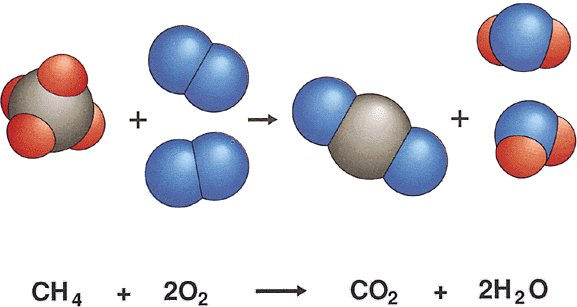
\includegraphics[width=2.64in,height=1.4in]{t11/media/image2.jpeg}\par}

Un ejemplo de reacción química es la formación de óxido de hierro
producida al reaccionar el oxígeno del aire con el hierro. Otro ejemplo
sería la combustión del metano.

Una reacción química también se puede entender como un proceso en el que
se rompen unos enlaces entre unos átomos y se forman otros diferentes.

En cada reacción química la relación en el número de moléculas de cada
sustancia que interviene es siempre la misma. A esta relación se le
llama \textbf{estequiometría.}

A la representación simbólica por escrito de una reacción química se le
llama \textbf{ecuación química.}

\hypertarget{ejemplos}{%
\subsubsection{Ejemplos}\label{ejemplos}}

\ch{CH4 (g) + O2 (g) -> CO2 (g) + H2O (g) + calor}

\ch{NH4SCN (s) + Ba(OH)2 (s) + calor -> Ba(SCN)2 (s) + NH3 (g) + H2O (l)}

\ch{NH3 (g) + HCl (g) -> NH4Cl (s)}

\hypertarget{leyes-ponderales}{%
\subsection{Leyes ponderales}\label{leyes-ponderales}}

En las reacciones químicas no se crean ni se destruyen átomos sino que
se cumple la \textbf{ley de Lavoisier de conservación de la masa} que
hemos visto en otros cursos (``la masa en un proceso químico no se crea
ni se destruye''), pues los átomos de cada elemento no cambian. Sólo
cambia su forma de unirse entre sí.

La \textbf{ley de Proust o ley de las proporciones definidas} dice que
cuando varias sustancias reaccionan para dar unos productos determinados
lo hacen siempre en unas proporciones fijas.

La \textbf{ley de las proporciones múltiples} afirma que cuando dos
elementos se combinan para originar distintos compuestos, se combinan
con dicha cantidad fija para dar como producto los compuestos, están en
relación de números enteros sencillos. Esta fue la última de las leyes
ponderales en postularse.

A diferencia de las anteriores, la \textbf{ley de los volúmenes de
combinación} propuesta por Gay-Lussac en 1809 relaciona los volúmenes de
los gases intervinientes en una reacción química. La ley establece que,
en una reacción en la que la temperatura y la presión son constantes,
los volúmenes de todos los gases que participan en ella guardan entre sí
una relación sencilla. Por ejemplo, Gay-Lussac descubrió que 2 volúmenes
de hidrógeno y 1 volumen de oxígeno que reaccionan forman 2 volúmenes de
vapor de agua.

\hfill\break{\centering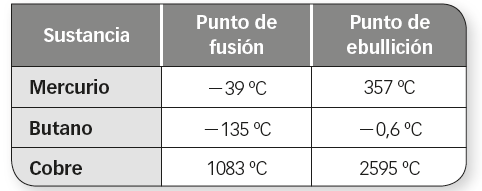
\includegraphics[width=3.12in,height=1.62in]{t11/media/image3.png}\par}

\hypertarget{cuxf3mo-se-escribe-una-reacciuxf3n-quuxedmica.-ajuste-de-ecuaciones-quuxedmicas}{%
\subsection{Cómo se escribe una reacción química. Ajuste de ecuaciones
químicas}\label{cuxf3mo-se-escribe-una-reacciuxf3n-quuxedmica.-ajuste-de-ecuaciones-quuxedmicas}}

Hacer que se cumpla le Ley de Lavoisier y la Ley de Proust en una
ecuación química es conseguir que el número de átomos de cada elemento
en los reactivos y en los productos sea el mismo. Al proceso con el que
logramos esto se denomina \textbf{ajuste de la ecuación química}.

Consiste en poner los coeficientes estequiométricos necesarios delante
de cada sustancia sin cambiar las fórmulas de cada una. Por ejemplo:

\ch{CH4 (g) + 2 O2 (g) -> CO2 (g) + 2 H2O (g)}

\ch{3 CH4 (g) + 6 O2 (g) -> 3 CO2 (g) + 6 H2O (g)}

Como vemos en el ejemplo, el ajuste no es único. Hay infinitos ajustes
correctos posibles.

\textbf{Ejercicios:}

\begin{exercise}Ajusta las siguientes ecuaciones:

\begin{enumerate}
\def\labelenumi{\alph{enumi})}
\item
  \ch{NH3 (g) + HCl (g) NH4Cl (s)}
\item
  \ch{C6H12O6 (s) -> C (s) + H2O (g)}
\end{enumerate}

\end{exercise}

\hypertarget{estequiometruxeda-buxe1sica}{%
\subsection{Estequiometría básica}\label{estequiometruxeda-buxe1sica}}

La \emph{estequiometría} es la parte de la Química que se ocupa de los
cálculos relacionados con las relaciones cuantitativas que se dan entre
los reactivos y los productos en el transcurso de una reacción química.

En una ecuación química ajustada, los coeficientes estequiométricos nos
indican las proporciones en moles entre las diferentes sustancias,
reactivos y productos que intervienen en una reacción química.

Por ejemplo en la reacción de combustión entre el metano y el oxígeno,
reacciona una molécula de metano con dos de oxígeno para dar una
molécula de dióxido de carbono y dos de agua. O lo que es lo mismo: un
mol de metano reacciona con dos moles de oxígeno para dar un mol de
dióxido de carbono y dos moles de agua.

En toda reacción química se debe conservar la masa pues el número de
átomos no cambia, solo cambia la forma de enlazarse. En el ejemplo
anterior ocurriría que \qty{16}{\g} de metano (\qty{1}{\mol}) reaccionan
con \qty{64}{\g} de oxígeno (\qty{2}{\mol}) para dar \qty{44}{\g} de
dióxido de carbono (\qty{1}{\mol}) y \qty{36}{\g} de agua
(\qty{2}{\mol}). (80g de reactivos dan 80g de productos: en todas las
reacciones químicas se tiene que cumplir siempre la ley de Lavoisier: la
masa se conserva).

En el laboratorio, en la industria, en la investigación, normalmente es
más útil conocer las proporciones en masa de las sustancias que
reaccionan. Para eso hemos de utilizar las masas molares de las
sustancias y utilizar la estequiometría en masa.

\textbf{Cálculos estequiométricos masa - masa}

En este tipo de cálculos, los datos están normalmente expresados en
gramos y la incógnita la piden también en gramos.

\textbf{Ejemplo}

El dióxido de manganeso reacciona con el cloruro de hidrógeno dando
dicloruro de manganeso, cloro y agua. Calcula los gramos de dicloruro de
manganeso que se obtienen cuando reaccionan \qty{7,5}{\g} de ácido
clorhídrico.

\emph{Resolución:}

Planteamos la ecuación: \ch{MnO2 + HCl -> MnCl2 + Cl2 + H2O}

La ajustamos: \ch{MnO2 + 4 HCl -> MnCl2 + Cl2 + 2 H2O}

Planteamos los cálculos indicando al principio lo que queremos obtener y
partimos del dato clave que son los gramos de HCl que reaccionan:

\[g\ \ch{MnCl2} = \qty{7,5}{\g}\ \ch{HCl} \cdot \frac{\qty{1}{\mol}\ \ch{HCl}}{\qty{36.5}{\g} \ch{HCl}} \cdot
\boxed{ \frac{\qty{1}{\mol} \ch{MnCl2}}{\qty{4}{\mol}\ \ch{HCl}} } \cdot \frac{\qty{126.0}{\g}\ \ch{MnCl2}}{\qty{1}{\mol}\ \ch{MnCl2}} = \qty{6.5}{\g}\ \ch{MnCl2}\]

\textbf{Ejercicios:}

\begin{exercise}Calcula los gramos de metano que podrán arder con 50
gramos de oxígeno para dar dióxido de carbono y agua. (S.
\qty{12,5}{\g})\end{exercise}

\begin{exercise}Quemamos \qty{0,486}{\g} de magnesio con oxígeno.
Calcula la masa del óxido obtenido. (S. \qty{0,81}{\g})\end{exercise}

\begin{exercise}El etanol se puede oxidar con oxígeno para dar ácido
acético y agua. Calcula la masa de ácido acético que se podrá obtener a
partir de \qty{10}{\g} de etanol. (S. \qty{13}{\g})\end{exercise}

\begin{exercise}El nitrato de amonio es un explosivo que a partir de
\qty{400}{\degreeCelsius} se descompone en monóxido de dinitrógeno y
vapor de agua. Plantea y ajusta la ecuación del proceso y calcula los
gramos de agua que se formarán en la descomposición de \qty{8,00}{\g} de
nitrato de amonio. (S. \qty{3,60}{\g}).\end{exercise}

\hypertarget{mecanismos-de-una-reacciuxf3n-quuxedmica-teoruxeda-de-las-colisiones-y-energuxeda-de-activaciuxf3n.}{%
\subsection{Mecanismos de una reacción química: Teoría de las colisiones
y energía de
activación.}\label{mecanismos-de-una-reacciuxf3n-quuxedmica-teoruxeda-de-las-colisiones-y-energuxeda-de-activaciuxf3n.}}

La teoría de colisiones considera que los cambios que ocurren en las
reacciones químicas se dan cuando las moléculas de reactivos chocan
entre ellas.

Sin embargo, \textbf{para producir reacción los choques han de ser
eficaces}. Los choques no son eficaces si no se dan con la energía
suficiente o con la orientación adecuada..

Por ejemplo, si tenemos una mezcla equimolecular de yodo e hidrógeno en
fase gaseosa en condiciones normales se calcula que se dan unos
10\textsuperscript{29} choques entre moléculas de \ch{I2} y de \ch{H2}
por cada segundo y por cada mL. Si todos los choques fueran eficaces la
reacción para dar yoduro de hidrógeno duraría del orden de
10\textsuperscript{--9}s, con velocidades del orden de
10\textsuperscript{6} mol/L·s. Sin embargo la reacción a temperatura
ambiente tiene una velocidad de 10\textsuperscript{-4}mol/L·s y puede
durar entre minutos y horas. Luego no todos los choques son eficaces.

\begin{figure}
\centering
\hfill\break{\centering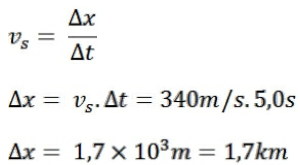
\includegraphics[width=4.72in,height=2.06in]{t11/media/image7.png}\par}
\caption{Resultado de imagen de choque eficaz gif}
\end{figure}

La causa está en que no todos los choques ocurren con la energía
necesaria (\textbf{energía de activación}) y tampoco lo hacen con la
orientación adecuada. Para la reacción anterior solo uno de cada
10\textsuperscript{14} choques es eficaz.

En la reacción \ch{I2 (g) + H2(g) -> 2 HI (g)} a temperatura ambiente
sólo una pequeña parte de las moléculas tiene la energía necesaria tal
que al chocar entre ellas puedan romper los enlaces de los reactivos y
formarse los enlaces de los productos.

A la energía mínima que tienen que tener las moléculas para que un
choque sea eficaz se le denomina \textbf{energía de activación
(\(E_a\))}.

Cuando tiene lugar una reacción química, inicialmente crece la energía,
al producirse la ruptura de los enlaces de los reactivos, hasta que se
alcanza un máximo.

El estado intermedio del sistema, al que corresponde la energía máxima,
se denomina \textbf{estado de transición o complejo activado.} La
energía necesaria para pasar desde los reactivos al estado de transición
se llama \textbf{energía de activación \(E_a\).}

Los reactivos deben superar la barrera de energía de activación para
poder convertirse en productos, incluso si la reacción fuese exotérmica.

El pico de la barrera corresponde al \textbf{complejo activado}, una
especie transitoria de visa muy corta que acaba dando lugar a los
productos.

Se reserva el término \textbf{catalizador} a las sustancias que aceleran
la velocidad de reacción; si la sustancia disminuye la velocidad de
reacción se denomina \textbf{inhibidor} o \textbf{catalizador negativo.}
La acción del catalizador se llama \textbf{catálisis}.

El catalizador no aparece en la ecuación neta de la reacción, ya que se
regenera en el transcurso de la misma.

\hfill\break{\centering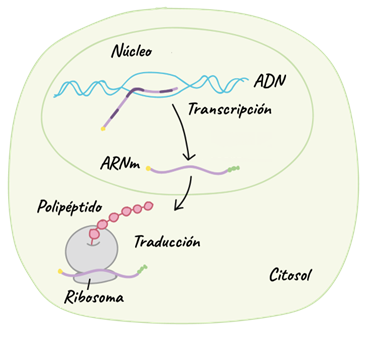
\includegraphics[width=4.3in,height=2.48in]{t11/media/image8.png}\par}

Los catalizadores aumentan la velocidad de reacción debido a que
disminuyen la energía de activación. El catalizador cambia el mecanismo
de la reacción: proporciona un camino de reacción alternativo, cuya Ea
será menor.

La presencia del catalizador no afecta en nada al calor de reacción ni a
la espontaneidad del proceso.

\hypertarget{cinuxe9tica-de-reacciuxf3n}{%
\subsection{Cinética de reacción}\label{cinuxe9tica-de-reacciuxf3n}}

Conocer qué factores afectan y de qué forma a la velocidad de las
reacciones químicas es importante para poder controlar la rapidez con la
que se dan.

Los factores principales que afectan a la velocidad de las reacciones
químicas y que vamos a estudiar son los siguientes:

\begin{itemize}
\tightlist
\item
  Estado físico y grado de división de los reactivos.
\item
  Concentración de los reactivos.
\item
  Temperatura.
\item
  Catalizadores.
\end{itemize}

\textbf{Estado físico y grado de división de los reactivos}

Como hemos visto en la teoría de colisiones, para que se de una reacción
química es necesario que los productos puedan realizar choques eficaces.
En los casos en que reaccione alguna sustancia sólida los choques se
realizarán en la superficie de las partículas sólidas y la velocidad
aumentará con la cantidad de superficie expuesta.

Por ello, \textbf{si reaccionan sustancias sólidas la velocidad
aumentará cuanto más pulverizado esté el sólido} pues entonces más
moléculas de reactivos podrán chocar unas con otras. Por ejemplo, el
carbón en polvo al arder lo puede hacer prácticamente con la rapidez de
un gas.

La harina en polvo puede arder en el aire con gran facilidad lo que en
ocasiones ha producido accidentes en industrias harineras.

En la reacción del mármol (carbonato de calcio) con el ácido clorhídrico
(disolución acuosa de cloruro de hidrógeno), con desprendimiento de
\ch{CO2}, la velocidad aumenta mucho al dividir el sólido en partículas
finas.

\[\ch{CaCO3 (s) + 2 HCl (ac) -> CaCl2 (ac) + CO2 (g) + H2O (l)}\]

La reacción del azúcar con clorato de potasio fundido es muy rápida y
muy exotérmica. ¿Qué pasaría si en vez de añadir una gominola sobre el
clorato de potasio fundido se añadiera azúcar en polvo? ¿Para que se
podría utilizar esa reacción de esta forma?

\[\ch{4 KClO3 (l) + C6H12O6 (s) -> 4 KCl (s) + 6 CO2 (g) + 6 H2O (l)}\]

El mayor grado de división y por tanto, la mayor facilidad para que
puedan entrar en contacto las moléculas de los reactivos se dará cuando
estos se encuentren en estado gaseoso o en disolución.

\textbf{Concentración de los reactivos}

\hfill\break{\centering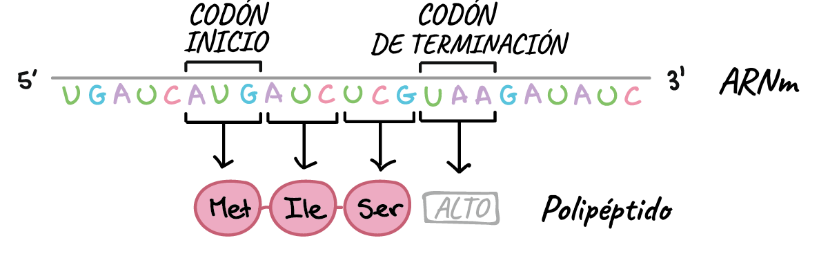
\includegraphics[width=1.7in,height=1.09in]{t11/media/image11.png}\par}

La frecuencia de los choques será mayor si la concentración de los
reactivos aumenta, es decir, será más fácil que se choquen las moléculas
de los reactivos cuantas más moléculas haya por unidad de volumen.

\textbf{Efecto de la temperatura}

Un aumento de la temperatura produce un aumento de la velocidad con que
se mueven las moléculas. Esto hace que el número de choques entre ellas
aumente.

Pero \textbf{un aumento de la temperatura} también \textbf{hace que un
mayor número de moléculas choquen con la energía adecuada} lo que hace
aumente el número de choques eficaces.

\textbf{La velocidad de una reacción aumenta con la temperatura.} Para
muchas reacciones se cumple aproximadamente que la velocidad se duplica
por cada \qty{10}{\degreeCelsius} que se aumenta la temperatura.

\textbf{Catalizadores}

Los catalizadores son sustancias que:

\begin{itemize}
\tightlist
\item
  \textbf{Aumentan mucho la velocidad de reacción}.
\item
  \textbf{Actúan en muy pequeñas cantidades}, no estequiométricas.
\item
  \textbf{No experimentan cambios químicos permanentes}, de forma que
  pueden recuperarse una vez finalizada la reacción.
\item
  \textbf{Alteran el mecanismo de la reacción disminuyendo la energía de
  activación} necesaria para formar los productos.
\item
  Los catalizadores \textbf{no cambian la estequiometría de una
  reacción.}
\end{itemize}

\hfill\break{\centering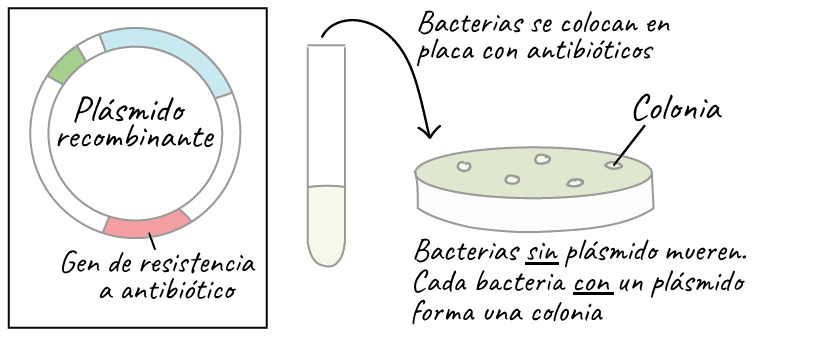
\includegraphics[width=1.75in,height=1.76in]{t11/media/image12.png}\par}

Por ejemplo, si tenemos: \ch{A + B -> AB}

Que puede ser catalizada por una sustancia E, lo que hace la sustancia E
es facilitar la formación de los productos pero a través de otro
mecanismo que requiere una energía de activación menor. Esto hace que la
reacción transcurra más rápidamente.

A la acción de los catalizadores en las reacciones químicas se la
denomina \textbf{catálisis}. Estudiaremos dos tipos principales:

\begin{itemize}
\item
  \textbf{Catálisis homogénea:} en ella los catalizadores están en el
  mismo estado físico (normalmente en fase líquida o gaseosa) que los
  reactivos sobre los que actúan.

  \[\ch{2 H2O2 (ac) -> 2 H2O (l) + O2 (g)}\]

  Un ejemplo de catálisis homogénea es la descomposición del peróxido de
  hidrógeno (agua oxigenada) que se cataliza por la adición de yoduro de
  potasio disuelto en el medio de reacción. La reacción global sería:
\item
  \textbf{Catálisis heterogénea:} los catalizadores están en diferente
  estado físico que los reactivos (normalmente los catalizadores están
  en estado sólido y los reactivos son líquidos o gases y la reacción
  catalizada se da en la superficie del catalizador). En la superficie
  del catalizador se pegan (adsorben los reactivos y es más fácil que
  reaccionen entre si para dar los productos.

  Un ejemplo de catálisis heterogénea sería la descomposición del agua
  oxigenada por la acción del óxido de manganeso (IV) sólido.

  \[\ch{2 H2O2 (ac) ->[ MnO2 (s) ] 2 H2O (l) + O2 (g)}\]

  Otro ejemplo es la siguiente reacción, que es muy lenta en fase
  gaseosa, pero que se da con gran rapidez en presencia de una pequeña
  cantidad de platino sólido, de la manera en que muestra la animación:

  \[\ch{2 NO (g) + 2 CO (g) ->[ Pt (s)] N2 (g) + 2 CO2 (g)}\]

  Otro ejemplo es la acción catalítica de metales nobles como el
  platino, el paladio y el rodio en los \textbf{catalizadores de los
  automóviles}. Hacen que los gases de escape contengan menos sustancias
  tóxicas al facilitarse su combustión completa.

  \[\ch{CO (g) + C_xH_y (g) + H2 (g) + O2 (g) ->[ Pt (s) ] CO2 (g) + H2O (g)}\]
  \[\ch{N_xO_y (g) ->[ Rh (s) ] N2 (g) + O2 (g)}\]

  Así los gases nocivos son convertidos en gases inocuos que pueden ser
  expulsados a la atmósfera.
\end{itemize}

\textbf{Ejercicio 6:} (Modelo EBAU 2024 Andalucía)

\hfill\break{\centering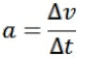
\includegraphics[width=6.52in,height=1.79in]{t11/media/image18.png}\par}

\hypertarget{clasificaciuxf3n-de-las-reacciones-quuxedmicas}{%
\subsection{Clasificación de las reacciones
químicas}\label{clasificaciuxf3n-de-las-reacciones-quuxedmicas}}

Según la forma de la reacción las reacciones químicas pueden
clasificarse en:

\textbf{Reacciones de análisis o de descomposición}: a partir de una
sustancia se forman otras más simples. Ejemplos:

Descomposición del azúcar por el efecto deshidratante del ácido
sulfúrico.

\[\ch{C6H12O6 ->[ H2SO4 (ac) ] 6 C + 6 H2O}\]

Descomposición del agua en la electrolisis

\[\ch{2 H2O (l) + energía~eléctrica -> 2 H2 (g) + O2 (g)}\]

Ya se está empezando a usar el hidrógeno producido a partir de energías
renovables como combustible de vehículos y para la industria.

\textbf{Reacciones de síntesis}: de varias sustancias se forma otra más
compleja. Ejemplos:

\ch{NH3 (g) + HCl(g) -> NH4Cl(s)}

\ch{N2H4 (g) + CO (s) -> CO(NH2)2 (s)}

Hay un tipo de reacciones de síntesis importantes denominadas reacciones
de formación.

Son aquellas en que una sustancia se forma a partir de sus elementos.
Ejemplos:

\ch{Mg (s) + 1/2 O2 (g) -> MgO (s)}

\ch{1/2 N2 (g) + 2 H2 (g) + 1/2 Cl2 (g) -> NH4Cl (s)}

\ch{2 H2 (g) + O2 (g) -> 2 H2O (l)}

\textbf{Reacciones de sustitución}: Un elemento se sustituye por otro en
un compuesto y lo deja libre. También se las denomina reacciones de
desplazamiento. Ejemplos:

\ch{HgCl2 (ac) + Cu (s) -> CuCl2 (ac) + Hg (s)}

\ch{2 AgNO3 (ac) + Cu (s) -> Cu(NO3)2 (ac) + Ag (s)}

\ch{HCl (ac) + Zn (s) -> ZnCl2 (ac) + H2 (g)}

\textbf{Reacciones de doble sustitución}: dos elementos o grupos se
intercambian entre dos compuestos. Se denominan también reacciones de
doble desplazamiento. Ejemplos:

\ch{Pb(NO3)2 (ac) + KI(ac) -> KNO3 (ac) + PbI2 (s)} (``lluvia de oro'')

\ch{AgNO3 (ac) + NaCl (ac) -> NaNO3 (ac) + AgCl (s)}

\hypertarget{importancia-de-las-transformaciones-quuxedmicas.}{%
\section{Importancia de las transformaciones
químicas.}\label{importancia-de-las-transformaciones-quuxedmicas.}}

\hypertarget{reacciones-quuxedmicas-de-transferencia-reacciones-redox-y-reacciones-uxe1cido-base.}{%
\subsection{Reacciones químicas de transferencia: reacciones redox y
reacciones
ácido-base.}\label{reacciones-quuxedmicas-de-transferencia-reacciones-redox-y-reacciones-uxe1cido-base.}}

En ellas se intercambian partículas pequeñas (iones o electrones) entre
diferentes sustancias. Las más importantes son las reacciones ácido-base
y las reacciones redox.

\hypertarget{reacciones-uxe1cido-base}{%
\subsubsection{Reacciones ácido-base}\label{reacciones-uxe1cido-base}}

También llamadas reacciones de transferencia de protones o reacciones de
neutralización: se transfieren protones, es decir, iones hidrógeno
(H\textsuperscript{+}) entre dos sustancias o iones. Son las reacciones
que se dan entre ácidos y bases. Ejemplos:

\ch{HCl + H2O -> Cl- + H3O+}

\ch{NH3 + H2O -> NH4+ + OH- -> NH4OH}

\ch{HCl + NH3 -> Cl- + NH4+ -> NH4Cl (s)}

En muchas ocasiones, en las reacciones ácido-base, se cumple que:

\textbf{ÁCIDO + BASE SAL + AGUA}

\emph{Ejemplo:} \ch{H2SO4 + 2 NaOH -> Na2SO4 + 2 H2O}

Las reacciones ácido-base se utilizan mucho para analizar disoluciones
de sustancias ácidas o básicas por la medida de los volúmenes que
reaccionan. A estas técnicas se les denomina \textbf{volumetrías
ácido-base} que veremos más adelante.

\textbf{Ácidos:} sustancias capaces de ceder protones
(H\textsuperscript{+}). Ejemplos: HCl, \ch{HNO3}, \ch{H2SO4}, ácido
acético, ácido fórmico, \ldots{}

\emph{Propiedades características de los ácidos}:

\begin{itemize}
\tightlist
\item
  Tienen sabor ácido.
\item
  Sus disoluciones conducen la corriente eléctrica.
\item
  Enrojecen el tornasol y decoloran la fenolftaleína.
\item
  Reaccionan con metales activos (Zn, Mg, \ldots) produciendo hidrógeno
  gaseoso.
\item
  Reaccionan con los carbonatos desprendiendo dióxido de carbono.
\item
  Reaccionan con las bases neutralizando sus propiedades.
\end{itemize}

\textbf{Bases:} sustancias capaces de coger protones
(H\textsuperscript{+}). Ejemplos: NaOH, \ch{Ca(OH)2}, \ch{NH3} \ldots{}

\emph{Propiedades características de las bases}:

\begin{itemize}
\tightlist
\item
  Tienen tacto jabonoso.
\item
  Sus disoluciones conducen la corriente eléctrica.
\item
  Colorean el tornasol de azul y la fenolftaleína de rosa.
\item
  Reaccionan con los ácidos neutralizando sus propiedades.
\end{itemize}

\textbf{Disoluciones ácidas, neutras y básicas}

En el agua, de forma natural, se da la siguiente reacción de
descomposición:

\[\ch{H2O (l) -> H+ (ac) + OH- (ac)}\]

Y en el agua siempre hay cierta cantidad de iones H\textsuperscript{+}
(iones hidrógeno o protones). En el agua pura, a
\qty{25}{\degreeCelsius} hay una concentración muy pequeña:
10\textsuperscript{-7} mol/litro. Si hay más de esa cantidad es porque
se ha añadido un ácido. Si hay menos es porque se ha añadido una base,
que ha hecho desaparecer parte de esos protones que tiene el agua de
forma natural.

La concentración de H\textsuperscript{+} puede variar mucho en una
disolución acuosa. Por ejemplo si es de 10\textsuperscript{-2} mol/litro
es porque se añadido un ácido. La concentración de protones, que se
representa por \${[}\ch{H^+}\$, en este caso sería 100.000 veces mayor
que en el agua pura. Si echáramos una base, la concentración de
H\textsuperscript{+} podría llegar a ser 10\textsuperscript{-14}
mol/litro: 10.000.000 veces menor que en el agua pura. Resumiendo:

\[\begin{array}{ll}
    [\ch{H^+}] = 10^{-7} \unit{\mol\per\L} & \Longrightarrow \text{disolución neutra} \\
    [\ch{H^+}] > 10^{-7} \unit{\mol\per\L} & \Longrightarrow \text{disolución ácida} \\
    [\ch{H^+}] < 10^{-7} \unit{\mol\per\L} & \Longrightarrow \text{disolución básica}
\end{array}\]

\textbf{Concepto de pH}

En biología, medicina, en la industria, etc. es muy importante poder
medir y expresar la concentración de H\textsuperscript{+} (iones
hidrógeno) que hay en un medio.

\[pH = - \log \left[\ch{H^^+} \right]\]

Para simplificar la medida de la cantidad de protones que hay en el agua
se usa mucho la escala de pH. Matemáticamente el pH es:

\hfill\break{\centering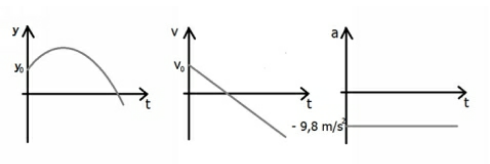
\includegraphics[width=3.46in,height=3.26in]{t11/media/image24.png}\par}

De forma simplificada esto quiere decir que cuando la concentración de
H\textsuperscript{+} es 10\textsuperscript{-2} \unit{\mol\per\L} el
\(pH=2\) y la disolución será muy ácida. Si
\(\ch{H^+} = 10^{-14} \unit{\mol\per\L}\) entonces el \(pH = 14\) y la
disolución será muy básica. Si el \(pH=7\) la disolución será neutra, es
decir, tendrá tantos protones como el agua pura.

La medida del pH se puede hacer de forma muy sencilla por medio de unos
colorantes denominados indicadores de pH, como la fenolftaleína o el
tornasol. También se usan papeles impregnados en esos colorantes que
cambian de color según el pH de la disolución. El más usado es el papel
indicador universal que se pone rojo en medios muy ácidos y azul en
medios muy básicos, pasando por toda una gama de colores intermedios.

Los aparatos electrónicos denominados \emph{peachímetros} (pH-metros)
nos dan el valor del pH de una disolución al sumergir en ella un
electrodo que llevan acoplado.

\begin{exercise}(Modelo EBAU Madrid 2024)

\end{exercise}

\hfill\break{\centering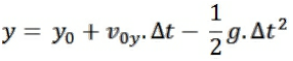
\includegraphics[width=6.69in,height=0.72in]{t11/media/image25.png}\par}

\hfill\break{\centering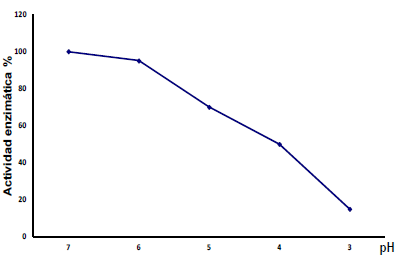
\includegraphics[width=4.26in,height=2.76in]{t11/media/image26.png}\par}

\hfill\break{\centering
\includegraphics[width=4.47in,height=0.21in]{t11/media/image27.png}\par}

\hfill\break{\centering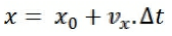
\includegraphics[width=6.69in,height=1.71in]{t11/media/image28.png}\par}

\hypertarget{reacciones-de-oxidaciuxf3n-reducciuxf3n}{%
\subsubsection{Reacciones de
oxidación-reducción}\label{reacciones-de-oxidaciuxf3n-reducciuxf3n}}

Se llaman también \textbf{reacciones de transferencia de electrones o
reacciones de oxidación -- reducción}. En estas reacciones algunos
átomos ganan o pierden electrones. \textbf{Se distinguen porque esos
átomos cambian sus números de oxidación}\emph{.} Se sabe planteando la
ecuación química y viendo el número de oxidación de cada elemento en los
reactivos y en los productos.

\emph{Ejemplos:} Combustión, fotosíntesis, oxidación de metales.

Cuando interviene el oxígeno, si aumenta la cantidad de oxígeno, se dice
que la sustancia se ha oxidado. Si disminuye la proporción de oxígeno,
decimos que se ha reducido.

\textbf{\emph{Oxidante}}: elemento de una sustancia que es capaz de
ganar electrones (e\textsuperscript{-}). Disminuye su número de
oxidación (se hace más negativo)

\textbf{\emph{Reductor}}: elemento de una sustancia capaz de ceder
e\textsuperscript{-}. Aumenta su número de oxidación (se hace más
positivo)

Ejemplo: \$\ch{C + }

El carbono pierde e\textsuperscript{-} \ch{0 -> + 4} (reductor)

El hierro gana e\textsuperscript{-} \ch{+ 3 -> 0} (oxidante)

Oxígeno: no pierde ni gana e\textsuperscript{--}

Las reacciones de oxidación son muy variadas y están en muchas facetas
de la vida normal. Las combustiones son oxidaciones; cuando nos
alimentamos oxidamos los alimentos en nuestras células para sacar
energía y poder vivir; los objetos de hierro se oxidan a la intemperie,
etc.

\begin{exercise}Ajusta las siguientes ecuaciones químicas y determina
qué elementos actúan como oxidantes y cuáles como reductores.

\begin{enumerate}
\def\labelenumi{\alph{enumi})}
\item
  \ch{F + O2 -> Fe2O3}
\item
  \ch{C + FeO -> Fe + CO2}
\item
  \ch{CH4 + O2 -> CO2 + H2O}
\item
  \ch{Na + H2O -> NaOH + H2}
\end{enumerate}

\end{exercise}

\hypertarget{procesos-industriales-medioambientales-y-sociales.}{%
\subsection{Procesos industriales, medioambientales y
sociales.}\label{procesos-industriales-medioambientales-y-sociales.}}

\hypertarget{la-problemuxe1tica-en-asturias}{%
\subsection{La problemática en
Asturias}\label{la-problemuxe1tica-en-asturias}}

Los principales procesos industriales relacionados con las
transformaciones químicas de Asturias, que veremos a continuación, son
los siguientes:

\begin{itemize}
\item
  \textbf{Bayer}

  Presenta en Langreo la planta donde se fabrican la mayoría de
  aspirinas del mundo. La aspirina es básicamente ácido
  acetilsalicílico, cuya reacción de síntesis es la siguiente:

  \hfill\break{\centering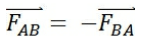
\includegraphics[width=4.94in,height=1.8in]{t11/media/image34.gif}\par}
\item
  \textbf{Arcelor-Mittal}

  La fabricación de acero se realiza en altos hornos, mediante una
  reacción que permite añadir carbono al mineral de hierro:

  \hfill\break{\centering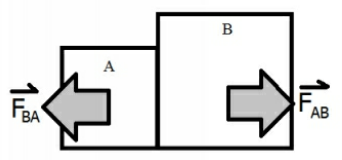
\includegraphics[width=0.75\textwidth,height=\textheight]{t11/media/image35.png}\par}
\item
  \textbf{Asturquimia}

  Originalmente una empresa familiar, llevan fabricando lejía desde hace
  más de un siglo en Asturias. Su iniciador y creador en el año 1928 se
  dio cuenta de que entre las muchas mercancías que vendía en su tienda
  en la ciudad de Oviedo, había una que destacaba por encima de las
  demás, ``La Lejía''.

  En aquella época, la elaboración de la lejía era muy pesada. Las
  materias primas, el cloruro de cal y las sosas, eran productos que
  desprendían gases durante su mezcla, la cual era muy laboriosa de
  llevar a cabo puesto que se hacia manualmente.
\item
  \textbf{Eumédica} (antigua Asturpharma)

  Se crea en diciembre de 1985 a partir de la reorganización empresarial
  de un importante grupo farmacéutico español con casi 100 años de
  tradición en los mercados farmacéuticos europeos.

  Tras años de dificultades financieras la empresa fue comprada en 2014
  por la multinacional Eumédica, que se dedica a la distribución de
  principios activos de antibióticos.
\item
  \textbf{Fertiberia}

  Dedicada a la fabricación de fertilizantes industriales para
  agricultura como nitrosulfato, nitrato de magnesio o los nitratos
  amónico-cálcicos.

  La fábrica de Avilés, que produce anualmente en torno a 600.000
  toneladas entre productos intermedios y finales, emplea a 137
  trabajadores.
\item
  \textbf{Maxam} (explosivos Trubia)

  La fábrica de municiones y armas de Trubia se levantó en 1794 porque
  se decidió instalar esa factoría en un paraje donde no estuviesen
  distantes los yacimientos de las materias primas a utilizar, como eran
  la madera, hierro y carbón.

  Famosa es la fabricación que tuvo del ``Carro ligero de Trubia'', el
  primero de diseño y construcción puramente españoles.

  \hfill\break{\centering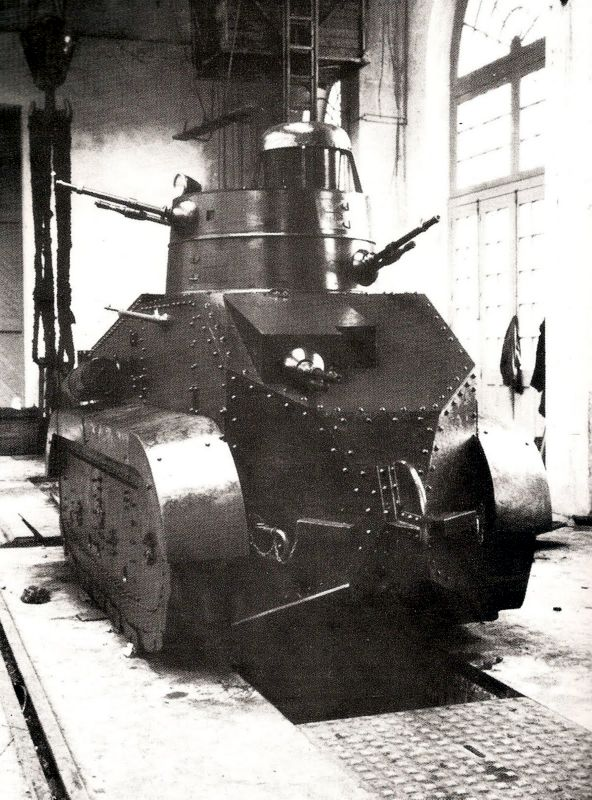
\includegraphics[width=2.78in,height=2.97in]{t11/media/image36.jpeg}\par}
\end{itemize}

\hypertarget{la-energuxeda-de-los-sistemas}{%
\section{La energía de los
sistemas}\label{la-energuxeda-de-los-sistemas}}

Antes de comenzar a hablar de la energía en los sistemas debemos dar
unas definiciones:

\textbf{Termodinámica:} parte de la Química-Física que estudia los
intercambios de energía entre los sistemas, principalmente aquellos en
los que interviene la energía térmica.

\textbf{Termoquímica:} parte de la Termodinámica en el que se consideran
las variaciones y los intercambios de energía en sistemas en los que se
producen reacciones químicas.

La Termoquímica es una parte de la ciencia común a la Física y a la
Química. La energía que se absorbe o se desprende en las reacciones
químicas suele tener mucho interés ya que algunas reacciones sólo las
realizamos para obtener energía como las combustiones. A veces esa
energía la convertimos en energía mecánica, como en los motores de
combustión.

\hypertarget{definiciuxf3n-de-energuxeda-y-ley-de-conservaciuxf3n-de-la-energuxeda.}{%
\subsection{Definición de energía y ley de conservación de la
energía.}\label{definiciuxf3n-de-energuxeda-y-ley-de-conservaciuxf3n-de-la-energuxeda.}}

Fuentes de energía en las reacciones químicas: calor y trabajo
termodinámicos.

\textbf{La energía interna de un sistema (U):} es la suma de todas las
energías que posee un sistema: química, térmica, nuclear, \ldots{} Sus
unidades son las unidades de energía: Julios, calorías, eV,\ldots{}

No podemos saber su valor total. En la energía interna no se tienen en
cuenta las energías cuyo valor depende de la posición del sistema con
respecto a otros cuerpos: energía cinética, potencial gravitatoria, etc.

\hfill\break{\centering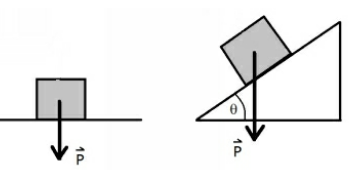
\includegraphics[width=3.03in,height=1.89in]{t11/media/image37.png}\par}

La variación de energía de un sistema en general la calcularemos
restando la energía inicial a la energía final, es decir, \textbf{la
energía interna es una función de estado}.

\[\Delta U = U_{final} - U_{inicial}\]

\(\Delta U\) será positiva si \(U_f > U_i\) y viceversa.

\begin{description}
\tightlist
\item[\textbf{Calor (Q)}]
energía que intercambia un sistema con el exterior debido a diferencias
de temperatura.
\item[\textbf{Trabajo (W)}]
energía que intercambia un sistema con el exterior debido a causas
distintas de las diferencias de temperatura: fuerzas gravitatorias,
fuerzas elásticas, diferencias de potencial eléctrico, etc.
\end{description}

\hfill\break{\centering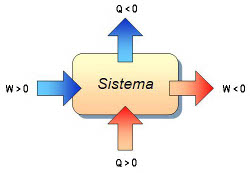
\includegraphics[width=2.18in,height=1.51in]{t11/media/image38.jpeg}\par}

Tanto el calor como el trabajo no son energías que posee un cuerpo sino
energías que entran o salen de un cuerpo, es decir, son variaciones en
la energía interna de un cuerpo. Sus unidades son las de la energía.

\textbf{Convenio de signos:} El trabajo y el calor son energías que gana
o pierde un sistema serán positivos si entran en el sistema y negativos
si salen.

El mismo calor que pierde un sistema lo puede ganar otro. El signo del
calor o del trabajo dependerán del sistema que consideremos.

\begin{description}
\tightlist
\item[\textbf{Ley de conservación de la energía}]
la cantidad total de energía en cualquier sistema físico aislado (sin
interacción con ningún otro sistema) permanece invariable con el tiempo,
aunque dicha energía puede transformarse en otra forma de energía.
\end{description}

En resumen, la ley de la conservación de la energía afirma que la
energía no se crea ni se destruye, solo se transforma, por ejemplo,
cuando la energía eléctrica se transforma en energía térmica en un
calefactor.

\hypertarget{definiciuxf3n-de-sistema-y-entorno.-tipos-de-sistemas-termodinuxe1micos}{%
\subsection{Definición de sistema y entorno. Tipos de sistemas
termodinámicos}\label{definiciuxf3n-de-sistema-y-entorno.-tipos-de-sistemas-termodinuxe1micos}}

\hfill\break{\centering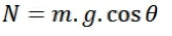
\includegraphics[width=2.07in,height=1.29in]{t11/media/image39.gif}\par}Hablamos
de \textbf{sistema termodinámico} como aquel sistema material en el que
consideramos los intercambios de materia y energía con el entorno.

Ejemplos de sistemas termodinámicos: la Tierra, la atmósfera, el cuerpo
humano, un lago, el cilindro de un motor, una bacteria, una estrella,
etc. Cualquier parte del Universo en el que consideremos el estudio de
las variaciones de energía que ocurren en su seno y entre él y el resto
del Universo será un sistema termodinámico.

\textbf{Tipos de sistemas termodinámicos}

\begin{itemize}
\item
  \textbf{Sistema termodinámico abierto}: el sistema que puede
  intercambiar materia y energía con el entorno.
\item
  \textbf{Sistema termodinámico cerrado}: el sistema que puede
  intercambiar energía con el entorno pero no materia.
\item
  \textbf{Sistema termodinámico aislado}: el sistema que no intercambia
  ni materia ni energía con el entorno.
\end{itemize}

\hfill\break{\centering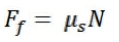
\includegraphics[width=4.43in,height=3in]{t11/media/image40.gif}\par}

Ejemplos: una reacción de combustión al aire libre, el cuerpo humano;
neutralización de ácido nítrico con hidróxido de sodio, una bombilla, un
termómetro, una olla a presión; agua en un calorímetro, un buzo en
neopreno, una bombona de butano, un iglú esquimal; etc.

\hypertarget{variables-termodinuxe1micas.-primera-ley-de-la-termodinuxe1mica.-aplicaciones.}{%
\subsection{Variables termodinámicas. Primera ley de la termodinámica.
Aplicaciones.}\label{variables-termodinuxe1micas.-primera-ley-de-la-termodinuxe1mica.-aplicaciones.}}

\textbf{El estado de un sistema} está definido por los valores de unas
magnitudes denominadas variables termodinámicas.

\textbf{Las variables termodinámicas de un sistema} son conjunto de
magnitudes macroscópicas que nos informan sobre las características y el
estado de ese sistema. Ejemplos:

\hfill\break{\centering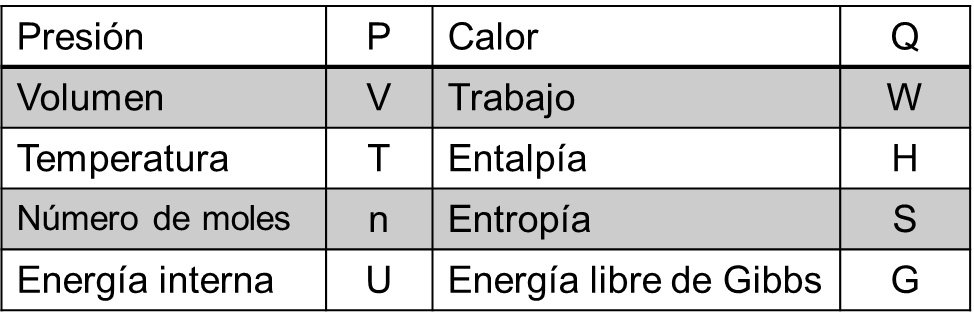
\includegraphics[width=3.7in,height=1.23in]{t11/media/image41.png}\par}

\hfill\break{\centering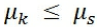
\includegraphics[width=1.97in,height=2.08in]{t11/media/image42.gif}\par}

Las variables termodinámicas de un sistema pueden ser:

\begin{itemize}
\item
  \textbf{Intensivas:} no dependen de la masa del sistema: T, P, ρ
  (densidad)
\item
  \textbf{Extensivas:} dependen de la masa del sistema: V, n, H
  (entalpía), U (energía interna)
\end{itemize}

\emph{Para saber si una magnitud es intensiva o extensiva basta con
imaginar si cambiaría su valor al dividir el sistema en dos partes.}

\hypertarget{funciones-de-estado}{%
\subsubsection{Funciones de Estado}\label{funciones-de-estado}}

\hfill\break{\centering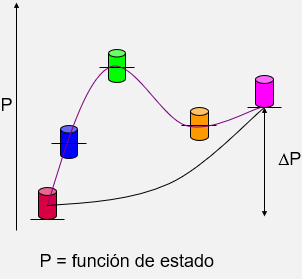
\includegraphics[width=2.36in,height=2.18in]{t11/media/image43.png}\par}

Son aquellas variables termodinámicas que tienen un valor definido para
cada estado del sistema y que no depende de las transformaciones que se
han llevado a cabo para llegar hasta ese estado.

\emph{Ejemplos}: presión, volumen, temperatura, energía interna, masa,
\ldots{}

Las variaciones de las funciones de estado dependen únicamente de los
valores de los estados inicial y final.

La variación de una función de estado entre dos instantes se puede
calcular al restar el valor inicial al valor final que tiene.

Al operar dos o más funciones de estado (suma, producto, etc.) el
resultado es otra función de estado.

\textbf{Funciones de estado: símiles mecánicos}

La altitud de un cuerpo respecto al nivel del mar, la masa de una
persona, la temperatura de un cuerpo, serían funciones de estado.

\[\Delta \text{masa} = \text{masa}_{final} - \text{masa}_{inicial} \qquad \Delta \text{altura} = \text{altura}_{final} - \text{altura}_{inicial}\]

La masa de alimentos ingerido por una persona, los kilómetros recorridos
por un corredor, el número de pasos que da una persona, el calor dado a
un cuerpo\ldots{} no serían funciones de estado

Si suponemos que un corredor corre a lo largo de una carretera siempre
en la misma dirección, los kilómetros recorridos se convertirían en
función de estado: se podrían hallar restando las dos posiciones del
corredor. Es decir, \textbf{algunas magnitudes que con rigor no son
funciones de estado, se pueden convertir en funciones de estado poniendo
ciertas condiciones a los cambios del sistema.}

\emph{La distancia recorrida se puede convertir en función de estado si
hacemos el ``truco'' de tomar siempre la posición a lo largo de la misma
trayectoria.}

\[\text{distancia recorrida} = \text{posición final} - \text{posición inicial}\]

\textbf{Ecuaciones de estado:} son fórmulas que relacionan varias
funciones de estado. A partir de los valores de unas funciones de estado
podemos calcular los valores de otras.

\emph{Ejemplos:} la ecuación de los gases ideales (\(PV = nRT\)), la
definición de entalpía (\(\Delta H = \Delta U + P\Delta V\)) o la
definición de la energía libre de Gibbs
(\(\Delta G = \Delta H - T\Delta S\))

\hypertarget{primera-ley-de-la-termodinuxe1mica}{%
\subsubsection{Primera ley de la
termodinámica}\label{primera-ley-de-la-termodinuxe1mica}}

No es ni más ni menos que el principio de conservación de la energía
expresado mediante conceptos usados en Termodinámica: energía interna,
calor y trabajo. Se puede enunciar de la siguiente manera:

\begin{quote}
\textbf{\emph{La variación de energía interna de un sistema cerrado es
igual a la suma del trabajo y del calor intercambiados con el entorno.}}
\end{quote}

\[\Delta U = Q + W\]

La energía interna de un sistema \textbf{es una función de estado} pero
el calor y el trabajo \textbf{no lo son}. No podemos calcular el trabajo
ni el calor que han sido intercambiados por un sistema mediante la
diferencia de ninguna magnitud presente en el sistema.

\hfill\break{\centering\includegraphics[width=2.23in,height=1.48in]{t11/media/image44.gif}\par}De
otra manera: Un sistema sólo tiene energía interna. Un sistema no
contiene calor o trabajo. Estos sólo existen durante un cambio
energético en el sistema. \textbf{El calor y el trabajo son energías en
tránsito debido a diferentes mecanismos}. La energía de un sistema
aislado permanece constante \[\Delta U = U_{final} - U_{inicial}\]
\[U_{B} - U_{A} = Q + W\]
\[\Delta U = U_{B} - U_A = Q_1 + W_1 = Q_2 + W_2 = Q_3 + W_3\]
\hfill\break{\centering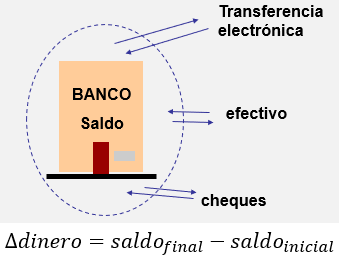
\includegraphics[width=2.35in,height=1.77in]{t11/media/image45.png}\par}
Podemos pensar un símil bancario de la energía interna de la siguiente
forma: el calor y el trabajo serían las distintas formas en que podemos
operar con nuestra cuenta bancaria: bizum, transferencias, enviar dinero
por Western Union\ldots{}

Todas las formas producen variaciones en el dinero de nuestra cuenta
(energía interna del sistema)

\textbf{Ejercicios:}

\begin{exercise}En una reacción química, un sistema absorbe del entorno
\qty{800}{\kJ} y realiza un trabajo de expansión de \qty{2}{\kJ}.
¿Cuánto ha variado su energía interna? (S. \qty{1340}{\J})\end{exercise}

\begin{exercise}Determina la variación de energía interna que sufre un
sistema cuando:

\begin{enumerate}
\def\labelenumi{\alph{enumi})}
\tightlist
\item
  Realiza un trabajo de \qty{600}{\J} y cede 40 calorías al entorno. (S.
  \qty{-767}{\J})
\item
  Absorbe 300 calorías del entorno y se realiza un trabajo de compresión
  de \qty{5}{\kJ}. (S. \qty{6250}{\J})
\end{enumerate}

\end{exercise}

\begin{exercise}En un recipiente cilíndrico con un émbolo móvil se
introducen 5 litros de un gas a \qty{1,4}{\atm} de presión. Si se le
suministran 200 calorías, manteniendo la presión constante, el gas se
expande hasta duplicar su volumen. ¿Qué variación de energía interna ha
experimentado el gas? (S. \qty{127}{\J})\end{exercise}

\hypertarget{introducciuxf3n-al-concepto-de-entalpuxeda.-entalpuxedas-de-reacciuxf3n.-diagramas-entuxe1lpicos.}{%
\subsection{Introducción al concepto de entalpía. Entalpías de reacción.
Diagramas
entálpicos.}\label{introducciuxf3n-al-concepto-de-entalpuxeda.-entalpuxedas-de-reacciuxf3n.-diagramas-entuxe1lpicos.}}

La Termoquímica nos permite predecir la cantidad de calor que liberan y
el trabajo que se puede realizar mediante una reacción química

La producción de energía mediante reacciones químicas forma parte de
nuestras vidas. El calor emitido por los combustibles al arder y la
energía que proporcionan los alimentos que ingerimos, están gobernados
por principios termodinámicos.

El calor de las reacciones químicas mueve el mundo, principalmente a
través de las reacciones de combustión.

En las reacciones químicas hay normalmente una absorción o liberación de
energía química que se transforma en otros tipos de energía (térmica,
eléctrica, luminosa, mecánica).

Las reacciones que desprenden energía se denominan \textbf{exotérmicas}
(\(\Delta H < 0\)). Las que la absorben se denominan
\textbf{endotérmicas} (\(\Delta H > 0\)).

\hypertarget{ecuaciones-termoquuxedmicas}{%
\subsubsection{Ecuaciones
termoquímicas}\label{ecuaciones-termoquuxedmicas}}

Una ecuación termoquímica es aquella ecuación química en la que se
indica la cantidad de energía que se absorbe o se desprende.

La cantidad de energía que se absorbe o desprende se puede indicar de
\textbf{dos maneras diferentes} que se muestran en los ejemplos. La
primera indica la energía como un reactivo o un producto más: si
necesitamos aportarla al inicio, será un reactivo; si aparece como
resultado de la reacción, será un producto. La segunda forma indica la
energía intercambiada empleando un término entálpico a la derecha de la
ecuación química, situado aparte. Esta última forma es la más común y la
que utilizaremos nosotros.

\[\begin{array}{lr}
    \text{Método 1}                               & \text{Método 2} \\
    \ch{C (s) + O2 (g) -> CO2 (g) + 393,5 kJ};    & \ch{C (s) + O2 (g) -> CO2 (g)} \quad \Delta H = \qty{-393,5}{\kJ} \\
    \ch{N2 (g) + O2 (g) + 180,7 kJ -> 2 NO (g)};  & \ch{N2 (g) + O2 (g) -> 2 NO (g)} \quad \Delta H = \qty{+180,7}{\kJ}
\end{array}\]

Los valores de energía que se indican se refieren siempre a las
cantidades de reactivos y productos en la ecuación ajustada en moles.
\[\ch{2 C(s) + 2 O2 (g) -> 2 CO2 (g) + 787 kJ}\] En los procesos
químicos la energía se debe conservar. Si arde una cantidad de hidrógeno
con oxígeno y se forma agua y se desprende energía, al descomponerse la
misma cantidad de agua debe de necesitarse la misma cantidad de energía.
\[\ch{H2 (g) + 1/2 O2 (g) -> H2O (l)} + \qty{285,8}{\kJ}\]
\[\ch{H2O (l) + 285,8 kJ -> H2 (g) + 1/2 O2 (g)}\]

\textbf{Ejercicios:}

\begin{exercise}El carbón de coque, o simplemente ``coque'', es un
combustible industrial muy importante muy usado en la industria
siderúrgica y del cemento. Procede del calentamiento, en ausencia de
aire, de carbones bituminosos con bajos contenidos en cenizas y en
azufre. Suponiendo que el coque es aproximadamente carbono puro y que se
cumple la ecuación termoquímica siguiente:
\[\ch{C (s) + O2 (g) -> CO2 (g)} + \qty{393,5}{\kJ}\] Calcula la energía
calorífica que se podría obtener en la combustión de una tonelada de
coque. (S. \qty{3,28e7}{\kJ})\end{exercise}

\begin{exercise}Para la obtención de oxigeno puro en el laboratorio se
utiliza la descomposición del clorato potásico según la reacción:
\[\ch{2 KClO3 (s) -> 2 KCl (s) + 3 O2 (g)} \qquad \Delta H^{0} = \qty{-89,5}{\kJ}\]
Calcula la energía calorífica que se desprende cuando se obtienen 20
litros de oxígeno medidos a \qty{25}{\degreeCelsius} y una atmósfera.
(S. \qty{24,4}{\kJ})\end{exercise}

\begin{exercise}La llamada reacción de la termita es muy exotérmica:
\[\ch{Fe2O3 (s) + 2 Al (s) -> Al2O3(s) + 2Fe(s)} \qquad \Delta H^{0} = \qty{-842}{\kJ}\]
Calcula la energía calorífica que se desprende cuando \qty{269,8}{\g} de
aluminio reaccionan con un exceso de óxido de hierro (III). (S.
\qty{-4210}{\kJ}).\end{exercise}

\hypertarget{entalpuxeda-de-reacciuxf3n}{%
\subsubsection{Entalpía de reacción}\label{entalpuxeda-de-reacciuxf3n}}

\hfill\break{\centering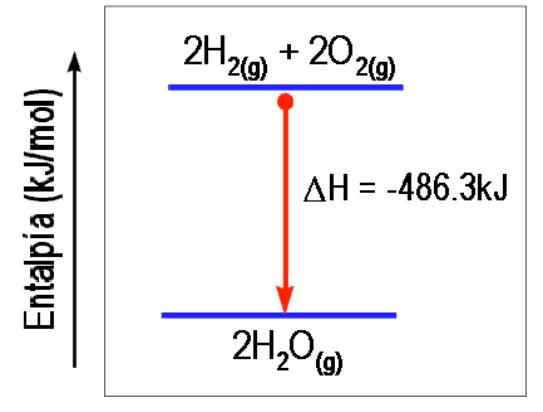
\includegraphics[width=2.98in,height=2.26in]{t11/media/image46.jpeg}\par}

La entalpía es una función de estado. Si consideramos una reacción
química que se desarrolla a presión constante, el calor que se absorbe o
se desprende en el sistema que reacciona es la variación de entalpía en
ese sistema cuando los reactivos se transforman en productos.

Dicho de otra manera, la energía que se absorbe o se desprende en una
reacción química a presión constante es la diferencia entre la entalpía
de los productos y la de los reactivos.

\[Q_{p} = \Delta H = H_\text{productos} - H_\text{reactivos}\]

\textbf{Entalpía estándar de reacción:} Para medir la variación de
entalpía de una reacción es muy cómodo elegir las condiciones a las que
se consideran los reactivos y los productos. Normalmente esas
condiciones son 1 atmósfera y \qty{25}{\degreeCelsius} (298K) y se
llaman condiciones estándar.

Las entalpías determinadas en esas condiciones se representan con un
``cerito'' similar al de grado centígrado:

\begin{itemize}
\item
  \textbf{H°} representa la entalpía de un sistema a
  \qty{25}{\degreeCelsius} y 1 atmósfera.
\item
  \textbf{∆H°} de un proceso representa la \emph{variación} de entalpía
  medida en condiciones estándar.
\end{itemize}

\[\ch{Reactivos (en condiciones estándar) -> Productos (en condiciones estándar)}\]

\[\Delta H^{0} = H_\text{productos}^{0} - H_\text{reactivos}^{0}\]

\hfill\break{\centering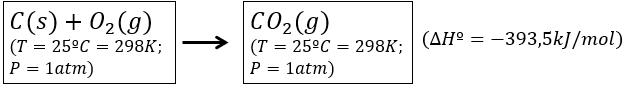
\includegraphics[width=6.56in,height=0.91in]{t11/media/image47.png}\par}

En el caso de las disoluciones se consideran condiciones estándar
\qty{25}{\degreeCelsius}, \qty{1}{\atm} y concentraciones \qty{1}{\M}
para las sustancias que intervengan en las reacciones.

La entalpía de reacción estándar (\(\Delta H_r^{0}\)) es la variación de
entalpía en una reacción cuando los reactivos, en sus estados estándar,
se transforman en los productos, en sus estados estándar, todo según los
correspondientes coeficientes estequiométricos.

\textbf{Ejemplo}

Si consideramos la descomposición del hidrogenocarbonato de sodio:
\[\ch{2 NaHCO3 (s) -> Na2CO3 (s) + H2O (l) + CO2 (g)}\]

Esto quiere decir que la descomposición térmica de 2 moles de
\ch{NaHCO3(s}) genera \qty{1}{\mol} de \ch{Na2CO3(s}), \qty{1}{\mol} de
\ch{H2O(l}) y \qty{1}{\mol} de \ch{CO2(g}), todos ellos en condiciones
estándar, con una variación energética a presión constante que es la
entalpía estándar de reacción ∆H\textsubscript{r}°.

\[\Delta H_{r}^{0} = H_{\ch{Na2CO3 (s)}}^{0} + H_{\ch{H2O(l)}}^{0} + H_{\ch{CO2(g)}}^{0} - 2H_{\ch{NaHCO3(s)}}^{0}\]

\textbf{Pero hay un gran problema}: no se puede saber el valor absoluto
de entalpía de ninguna sustancia.

\hypertarget{diagramas-entuxe1lpicos.-entalpuxeda-estuxe1ndar-de-reacciuxf3n.}{%
\subsection{Diagramas entálpicos. Entalpía estándar de
reacción.}\label{diagramas-entuxe1lpicos.-entalpuxeda-estuxe1ndar-de-reacciuxf3n.}}

\hypertarget{diagramas-entuxe1lpicos}{%
\subsubsection{Diagramas entálpicos}\label{diagramas-entuxe1lpicos}}

Para las reacciones químicas se suelen representar las variaciones de
entalpía mediante diagramas en donde se representa el nivel de energía
(entalpía) de reactivos y productos y el cambio que se da en la reacción
química. Si la entalpía decrece es que se libera energía y la reacción
será exotérmica y viceversa:

\hfill\break{\centering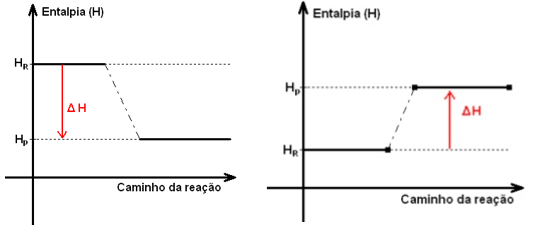
\includegraphics[width=5.59in,height=2.34in]{t11/media/image48.png}\par}

Por esto es más frecuente escribir las ecuaciones termoquímicas con un
tercer ``término entálpico'' de la siguiente forma, tal como estudiamos
anteriormente \[\ch{Reactivos -> Productos} \quad \Delta H_{r}^{0}\]

En los diagramas entálpicos se distingue muy bien por su forma cuando un
proceso es exotérmico (∆H°\textless0) o endotérmico (∆H°\textgreater0).

En abscisas se representa lo que se suele denominar ``coordenada de
reacción'', ``progreso de la reacción'' o ``camino de reacción'', que
está relacionado con el tiempo y al que no se le asigna ninguna escala.
Solo nos indica que la reacción progresa desde los reactivos
(normalmente a la izquierda) hacia los productos (normalmente a la
derecha en el diagrama).

\textbf{Ejemplos:}

Los diagramas entálpicos siguientes corresponden a las ecuaciones
termoquímicas que se indican al lado.

\hfill\break{\centering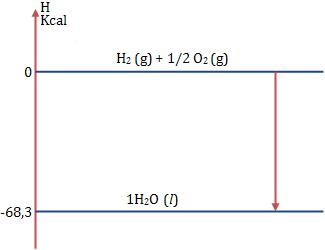
\includegraphics[width=1.89in,height=1.45in]{t11/media/image49.jpeg}\par}

\[\ch{H2 (g) + 1/2 O2 (g) -> H2O (l)} \qquad \Delta H^{0} = \qty{-68,3}{\kcal}\]

\hfill\break{\centering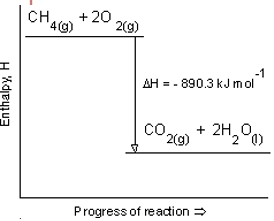
\includegraphics[width=2.16in,height=1.74in]{t11/media/image50.png}\par}

\[\ch{CH4 + 2 O2 -> CO2 + 2 H2O} \qquad \Delta H^{0} = \qty{-890,3}{\kJ}\]

\hfill\break{\centering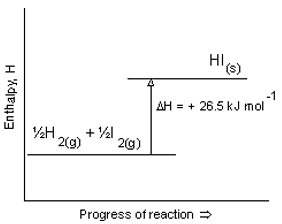
\includegraphics[width=2.29in,height=1.82in]{t11/media/image51.png}\par}

\[\ch{1/2 H2 + 1/2 I2 -> HI} \qquad \Delta H^{0} = \qty{+26,5}{\kJ}\]

\textbf{Ejercicio:}

\begin{exercise}Sabiendo que la reacción
\ch{2 HgO (s) -> 2 Hg (l) + O2 (g)} tiene una entalpía de reacción
\(\Delta H_{r}^{0} = \qty{+181,6}{\kJ}\) a \qty{25}{\degreeCelsius} y
\qty{1}{\atm} de presión:

\begin{enumerate}
\def\labelenumi{\alph{enumi})}
\tightlist
\item
  Dibuja esquemáticamente su diagrama de entalpía e indica si la
  reacción es endotérmica o exotérmica. ¿Cuánta energía se intercambia
  al descomponer \qty{100}{\g} de HgO? (S. \qty{41,9}{\kJ})
\item
  ¿Cuántos litros de oxígeno se obtienen, medidos a
  \qty{46}{\degreeCelsius} y \qty{1,5}{\atm}, en el proceso anterior?
  (S. \qty{4,0}{\L} de \ch{O2})
\end{enumerate}

\end{exercise}

\hypertarget{entalpuxeda-de-formaciuxf3n}{%
\subsubsection{Entalpía de
formación}\label{entalpuxeda-de-formaciuxf3n}}

Es el incremento entálpico (ΔH) que se produce en la reacción de
formación de un mol de un determinado compuesto a partir de los
elementos en el estado físico normal (en condiciones estándar). Los
elementos tienen una entalpía de formación de 0.

Las entalpías de formación nos dan cierta idea de la estabilidad de una
sustancia. Si al formarse una sustancia a partir de sus elementos se
desprende mucha energía esto significa que es una sustancia muy estable.
Si hay que dar energía para que se forme, esa sustancia tenderá a
descomponerse y desprender esa energía.

Los valores para la entalpía de formación de distintos compuestos están
tabulados, algunos de los más usuales son:

\hfill\break{\centering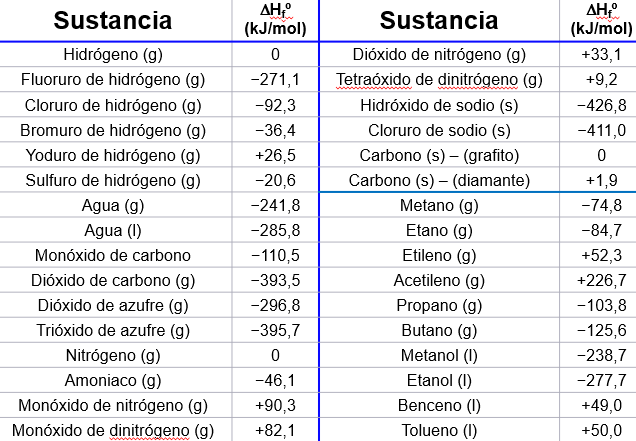
\includegraphics[width=6.62in,height=4.59in]{t11/media/image52.png}\par}

Se expresa como ΔH\textsubscript{f}\textsuperscript{0}. Se trata de un
``calor molar'', es decir, el cociente entre
ΔH\textsubscript{f}\textsuperscript{0} y el número de moles formados de
producto. Por tanto, se mide en kJ/mol.

A partir de los valores de las entalpías de formación de las sustancias
que intervienen en cualquier reacción se puede calcular fácilmente el
valor de la entalpía de esa reacción sin necesidad de realizar la
medición experimental.

Ejemplos:
\(\ch{C (s) + O2 (g) -> CO2 (g)} \qquad \Delta H_f^0 = \qty{-393,13}{\kJ\per\mol}\)

\(\ch{H2 (g) + 1/2 O2 (g) -> H2O (l)} \qquad \Delta H_f^0 = \qty{-285,8}{\kJ\per\mol}\)

Por definición de entalpía estándar de formación los valores de las
entalpías de formación de cualquier elemento en condiciones estándar es
cero. Esto lo hemos de tener en cuenta en los cálculos y los simplifica
mucho.

En general para cualquier reacción se cumple:

\[\Delta H_{reacción}^{0} = \sum n_{p}\Delta H_{f}^{0}(productos) - \sum n_{r}\Delta H_{f}^{0}(reactivos)\]

Siendo \(n_p\) y \(n_r\) los coeficientes estequiométricos
correspondientes a los productos y reactivos, respectivamente.

Esta fórmula tiene la ventaja de que, conociendo los valores de las
entalpías de formación de las sustancias que intervienen en cualquier
reacción química, podremos siempre calcular su entalpía de reacción
mediante una simple operación algebraica.

\textbf{Ejercicios:}

\begin{exercise}Plantea las ecuaciones necesarias para hallar el calor
de combustión del alcohol etílico (etanol) que se representa en el
siguiente diagrama entálpico. Calcula el calor molar estándar de
combustión con los datos necesarios obtenidos de la tabla de entalpías
estándar de formación. (S. \qty{-1366,7}{\kJ\per\mol})\end{exercise}

\begin{exercise}Calcula el calor que se desprenderá al quemar 1 litro de
alcohol etílico puro cuya densidad es \qty{0,78}{\g\per\mL}. (S.
\qty{-23174}{\kJ})\end{exercise}

\hypertarget{introducciuxf3n-a-la-entropuxeda.-segundo-y-tercer-principio-de-la-termodinuxe1mica.}{%
\subsection{Introducción a la entropía. Segundo y Tercer principio de la
termodinámica.}\label{introducciuxf3n-a-la-entropuxeda.-segundo-y-tercer-principio-de-la-termodinuxe1mica.}}

Hay muchos procesos en la naturaleza que son predecibles. Ocurren
siempre de la misma manera: en las cascadas el agua siempre cae
espontáneamente hacia abajo, los cuerpos calientes tienden a enfriarse
espontáneamente cediendo calor al ambiente, los gases tienden
espontáneamente a ocupar todo el espacio disponible en el recipiente que
los contiene.

Nunca se ha visto que espontáneamente en los ríos el agua fluya
espontáneamente curso arriba o que un café caliente se vuelva más
caliente a expensas de enfriar al ambiente, aunque se conserve la
energía. Si en alguna película vemos esto pensamos enseguida que la
película se ha proyectado al revés. Hay procesos que sabemos por
experiencia que no ocurren espontáneamente.

En general hay una tendencia en el universo a que los sistemas
evolucionen hacia la mínima energía (procesos exotérmicos).

Sin embargo hay procesos que ocurren de forma espontánea y son
endotérmicos, es decir, ocurren aumentando la energía de un sistema. El
hielo tiende a fundirse cogiendo calor del ambiente. El alcohol tiende
también a coger energía del ambiente y evaporarse. Al disolverse algunas
sales como el nitrato de amonio en agua el sistema coge calor del
ambiente. En todos estos casos se ha visto que aumenta el desorden.

Hay una tendencia a que aumente de forma espontánea el desorden de los
sistemas.

Un proceso \textbf{espontáneo} es aquel que tiene lugar sin la
aplicación de un agente externo; es decir, se produce de manera
espontánea en las condiciones en las que se encuentra el sistema. Si se
necesita una modificación en la temperatura, o en la presión, o el
aporte de una energía inicial, el proceso se considera \textbf{no
espontáneo} en esas condiciones.

Si dejamos escapar el gas que hay en una bombona por una habitación es
muy poco probable que vuelvan todas las moléculas a juntarse donde
estaban al principio, es decir tienden al desorden. No es imposible,
pero es tremendamente improbable. \textbf{Los sucesos tienden al máximo
desorden que es el estado de máxima probabilidad}.

En termodinámica el grado de desorden de un sistema se puede medir
mediante una magnitud que se denomina \textbf{entropía} (S) cuyas
unidades son \unit{\J\per\K}

La entropía, es decir, el desorden de un sistema, aumenta al pasar de
sólido a líquido y de líquido a gas. En general \textbf{la entropía
aumenta cuando un sistema recibe calor}. La cantidad de calor que ha
recibido un sistema nos dirá el aumento de entropía que ha sufrido.

\hfill\break{\centering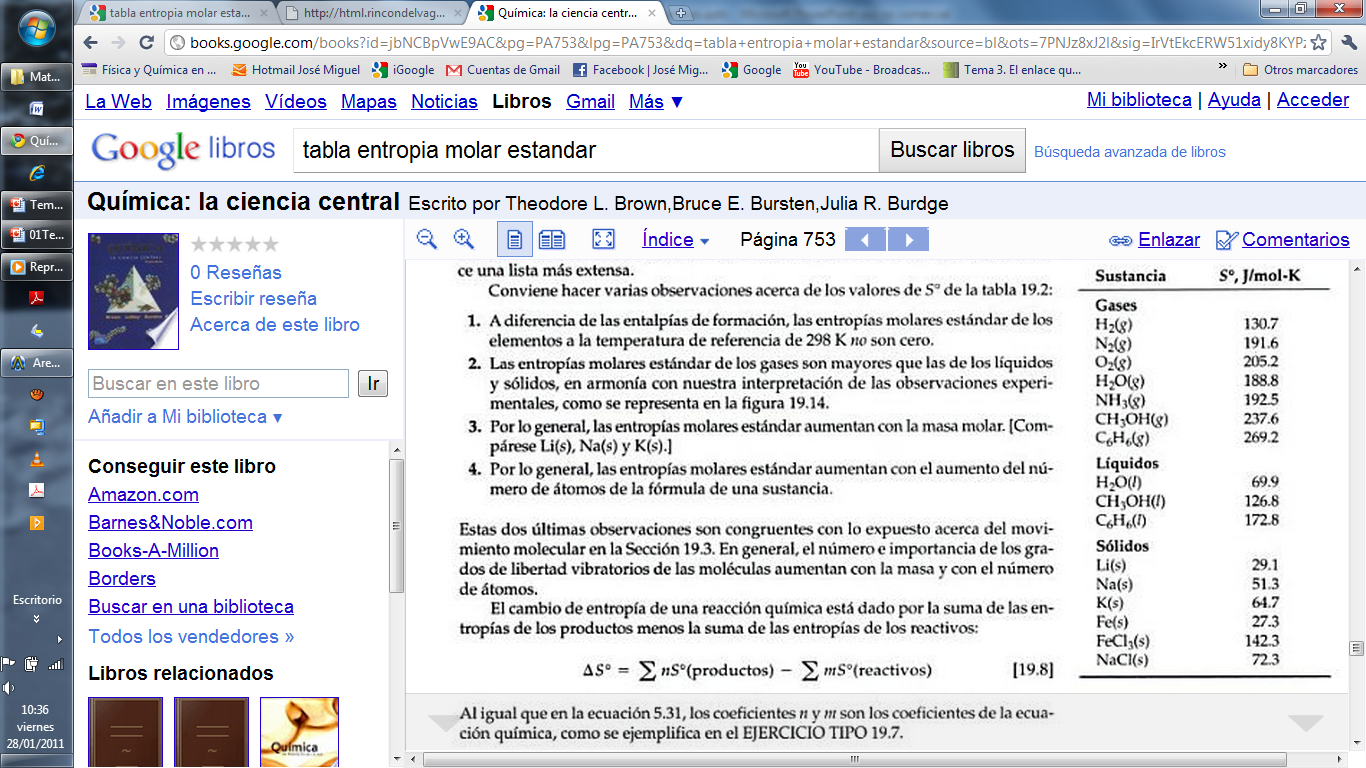
\includegraphics[width=1.78in,height=2.65in]{t11/media/image53.png}\par}

Se considera que una sustancia en el cero absoluto en forma de cristal
perfecto tiene un orden perfecto y entonces se le asigna una entropía
nula \textbf{\emph{(tercer principio de la termodinámica).}}

A partir de ahí se puede pensar que para desordenarlo le podemos dar
calor. La variación de la entropía de un sistema al recibir calor a una
temperatura constante se mide con la expresión:

\[\Delta S = \frac{Q}{T}\]

Si la temperatura no es contante para hallar la entropía de una
sustancia a una temperatura T se usa la expresión:

\[S = \int_{0}^{T}\frac{dQ}{T}\]

Por tanto, \textbf{se puede conocer el valor de la entropía que tiene
una sustancia en unas condiciones determinadas.} Existen tablas con
valores de entropía molar estándar de diferentes sustancias. Son las
llamadas entropías de un mol de una sustancia a \qty{25}{\degreeCelsius}
y \qty{1}{\atm}, simbolizadas por S\textsuperscript{0}. Las entropías de
los elementos en condiciones estándar (S\textsuperscript{0}) no son 0
sino que son siempre positivas.

Como en el caso de las entalpías de formación, gracias a los valores
tabulados se puede conocer la variación de la entropía en cualquier
reacción química en condiciones estándar mediante la siguiente
expresión:

\[\Delta S^0 = \sum n_p S_\text{productos}^0 - \sum n_r S_\text{reactivos}^0\]

\textbf{Ejemplo:}

Calcula ∆S\textsuperscript{0} para las siguientes reacciones químicas:

\begin{enumerate}
\def\labelenumi{\alph{enumi})}
\item
  \ch{N2 (g) + O2 (g) -> 2 NO (g)};
\item
  \ch{3 H2 (g) + N2 (g) -> 2 NH3 (g)}
\end{enumerate}

\emph{Datos:} de entropías molares estándar (S\textsuperscript{0}) en
\unit{\J\per\mol\per\K}:

\(\ch{H2 (g)} = 130,6\); \(\ch{O2 (g)} = 205\); \(\ch{N2 (g)} = 191,5\);
\(\ch{NO (g)} = 210,7\); \(\ch{NH3 (g)} = 192,3\).

\textbf{Resolución:}

\[\Delta S^0 = \sum n_p S_\text{productos}^0 - \sum n_r S_\text{reactivos}^0\]

\begin{enumerate}
\def\labelenumi{\alph{enumi})}
\tightlist
\item
  \(\Delta S^0 = \qty{2}{\mol} \cdot \qty{210,7}{\J\per\mol\per\K} - ( \qty{191,5}{\J\per\K} + \qty{205}{\J\per\K} ) = \qty{24,9}{\J\per\K}\)
\item
  \(\Delta S^0 = 2 \cdot \qty{192,3}{\J\per\K} - (\qty{3}{\mol} \cdot \qty{130,6}{\J\per\mol\per\K} + \qty{191,5}{\J\per\K} ) = \qty{-198,7}{\J\per\K}\)
\end{enumerate}

\textbf{Ejercicios:}

\begin{exercise}Calcula la variación de entropía al formarse \ch{H2O}
(l) a partir de \ch{H2} (g) y \ch{O2} (g).

\emph{Datos:} S° \ch{H2} (g) = \qty{130,7}{\J\per\mol\per\K}; S° \ch{O2}
(g) = \qty{204,8}{\J\per\mol\per\K}; S° \ch{H2O} (l) = 69,8\#J/mol/K*

\emph{Solución: - \qty{163,3}{\J\per\mol\per\K}}\end{exercise}

\begin{exercise}Halla la variación de entropía que tiene lugar en la
combustión en condiciones estándar del etanol.

\emph{Datos:} S° \ch{CO2(g}) = 213,8 J/mol K; S° \ch{CH3-CH2OH} (l) =
160,5 J/mol K;

\emph{S° \ch{H2O} (l) = \qty{69,8}{\J\per\mol\per\K}; S° \ch{O2} (g) =
\qty{204,8}{\J\per\mol\per\K}}

\emph{Solución: \qty{-137,9}{\J\per\mol\per\K}}\end{exercise}

\hypertarget{segundo-principio-de-la-termodinuxe1mica}{%
\subsubsection{Segundo principio de la
termodinámica}\label{segundo-principio-de-la-termodinuxe1mica}}

La entropía es una variable macroscópica que nos mide el grado de
desorden microscópico de un sistema. Es una función de estado. Su
variación entonces solo depende de la situación entrópica inicial y
final del sistema y no de los pasos intermedios:

\[\Delta S = S_{final} - S_{inicial}\]

\hfill\break{\centering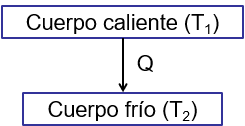
\includegraphics[width=2.24in,height=1.5in]{t11/media/image54.png}\par}\textbf{¿Qué
ocurre cuando dos cuerpos a diferente temperatura se ponen en contacto?}

Cuando dos cuerpos a diferente temperatura se ponen en contacto siempre
el calor Q pasa del más caliente al más frío. Si suponemos que cada
cuerpo mantiene su temperatura en el proceso las variaciones de entropía
serían:

\[\Delta S_{1} = \frac{Q}{T_{1}} < 0;\Delta S_{2} = \frac{Q}{T_{2}} > 0\]

Como \(T_1 > T_2\) entonces:
\(\left| \Delta S_{1} \right| < \left| \Delta S_{2} \right|\)

Y ocurre que la variación total de entropía al pasar el calor entre los
dos cuerpos a diferente temperatura: \(\Delta S_{1} + \Delta S_{2} > 0\)

\textbf{¡Y la entropía total ha aumentado!}

Todo esto nos conduce al \textbf{2º principio de la termodinámica:}

\begin{quote}
\textbf{La entropía es una magnitud cuyo valor total siempre tiende a
aumentar en los procesos espontáneos que se dan en la naturaleza.}
\end{quote}

Puede haber sistemas que se ordenen, es decir, que pierdan entropía, que
aumenten su orden a expensas de otros, pero la entropía del Universo
siempre aumentará.

\[\Delta S_\text{universo} = \Delta S_\text{sistema} + \Delta S_\text{entorno} \ge 0\]

El segundo principio de la termodinámica también se puede enunciar como:
``en los procesos reversibles la entropía del universo se mantiene
constante; en los procesos irreversibles la entropía del universo
siempre aumenta''.

Un \textbf{proceso reversible} es aquel que puede invertirse a la
situación anterior mediante un cambio infinitesimal en las condiciones
externas; es decir, las variables que definen el sistema pueden cambiar
de manera que cuando el proceso sea invertido, estas pasen por los
mismos valores en orden inverso. Si esa posibilidad no puede realizarse,
el proceso se considera \textbf{irreversible}.

Como según este principio la entropía del universo aumenta durante un
proceso espontáneo pueden darse procesos en que un sistema se vuelva más
ordenado (disminuya su entropía) siempre que el entorno aumente su
desorden y en conjunto la entropía total del universo se incremente.
Para que esto ocurra, la reacción química debe ser forzosamente
exotérmica, de manera que el calor que libera al entorno produzca un
incremento de entropía superior a lo que ha disminuido en el interior
del sistema.

\hfill\break{\centering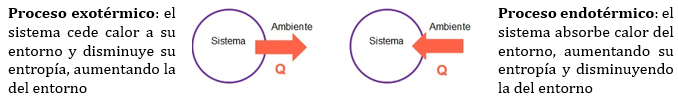
\includegraphics[width=6.79in,height=1.02in]{t11/media/image55.png}\par}

Pero en ambos casos se cumple:
\(\Delta S_\text{universo} = \Delta S_\text{sistema} + \Delta S_\text{entorno} \ge 0\)

En procesos reversibles a temperatura constante se puede calcular
\(\Delta S\) de un sistema así:

\[\Delta S = \frac{Q_\text{reversible}}{T}\]

Si consideramos procesos reversibles a temperatura y presión constante
el calor intercambiado será la variación de entalpía y se puede calcular
∆S de un sistema como:

\[\Delta S = \frac{\Delta H}{T}\]

La entropía del sistema aumenta si:

\begin{itemize}
\tightlist
\item
  Las sustancias pasan de sólido a líquido o de líquido a gas.
\item
  Se forma un mayor número de moles de sustancias gaseosas.
\item
  Se dan procesos de disolución de sólidos en líquidos
\item
  En la reacción no intervienen sustancias gaseosas, pero existe un
  aumento considerable en el número de moles de los productos respecto
  al de los reactivos.
\end{itemize}

\textbf{Ejercicio:}

\begin{exercise}Indica el signo de la variación de entropía que cabe
esperar en las siguientes reacciones:

\begin{enumerate}
\def\labelenumi{\alph{enumi})}
\item
  \ch{CaCO3 (s) -> CaO (s) + CO2 (g)}
\item
  \ch{HCl (g) + NH3 (g) -> NH4Cl (s)}
\item
  \ch{2 HCl (aq) + Zn (s) -> ZnCl2 (aq) + H2 (g)}
\item
  \ch{CuSO4 · 5 H2O (s) -> CuSO4 (aq) + 5 H2O (l)}
\end{enumerate}

\end{exercise}

\hypertarget{problemas-relacionados-con-el-consumo-energuxe9tico.-problemuxe1tica-en-asturias.}{%
\subsection{Problemas relacionados con el consumo energético.
Problemática en
Asturias.}\label{problemas-relacionados-con-el-consumo-energuxe9tico.-problemuxe1tica-en-asturias.}}

\newpage
\xsimsetup{
  solution/template = {gedmargin-solution},
  solution/name     = {S},
  }
{\small \printsolutions}


\end{document}
